%% =============================================================
%%  Les tonalités — des tons voisins aux modes anciens
%%  Guide de référence, composé en LaTeX, gravures LilyPond
%% =============================================================
%%
%%  Les figures (gravures/t-*.cropped.pdf), le cercle des quintes,
%%  le tableau des modes sur ré, les réponses des exercices
%%  (gravures/tonalites-*.tex) et le fichier tonalites.musicxml sont
%%  produits par outils/generer_tonalites.py, à partir du modèle de
%%  hauteurs des autres guides (outils/gammes.py). Voir le colophon
%%  en dernière page.
%%
\documentclass[a4paper,11pt]{article}

\usepackage[top=2.2cm,bottom=2.4cm,left=2.2cm,right=2.2cm]{geometry}
\usepackage[T1]{fontenc}
\usepackage[utf8]{inputenc}
\usepackage[french]{babel}
\usepackage{lmodern}
\usepackage{xcolor}
\usepackage{graphicx}
\usepackage{titlesec}
\usepackage{fancyhdr}
\usepackage{mdframed}
\usepackage{array}
\usepackage{enumitem}
\usepackage{booktabs}
\usepackage{tikz}
\usepackage{needspace}
\usepackage{hyperref}

\graphicspath{{gravures/}}

% ---- Couleurs, reprises du document des accords de guitare ---------
\definecolor{navy}{RGB}{18,50,105}
\definecolor{lightnavy}{RGB}{235,241,255}
\definecolor{mygray}{RGB}{110,110,110}
\definecolor{accent}{RGB}{150,40,30}

\hypersetup{colorlinks=true, linkcolor=navy, urlcolor=navy,
  pdftitle={Les tonalités — des tons voisins aux modes anciens},
  pdfauthor={Fabian Bastin}}

% ---- En-tête et pied -----------------------------------------------
\pagestyle{fancy}
\fancyhf{}
\renewcommand{\headrulewidth}{0.4pt}
\renewcommand{\footrulewidth}{0.4pt}
\fancyhead[L]{\small\bfseries\textcolor{navy}{Les tonalités}}
\fancyhead[R]{\small\textcolor{mygray}{\thepage}}
\fancyfoot[C]{\small\textcolor{mygray}{Des tons voisins aux modes anciens}}

% ---- Titres de section ---------------------------------------------
\newcommand{\navysect}[1]{%
  \colorbox{navy}{%
    \parbox[c][17pt]{\dimexpr\linewidth-2\fboxsep\relax}{%
      \color{white}\hspace{6pt}\bfseries\normalsize #1}}%
}
\titleformat{\section}[block]{\normalfont}{}{0pt}{\navysect}
\titlespacing*{\section}{0pt}{16pt}{10pt}

% ---- Encadré de remarque -------------------------------------------
\newmdenv[linecolor=navy, linewidth=0.5pt, backgroundcolor=lightnavy,
  innertopmargin=6pt, innerbottommargin=6pt,
  innerleftmargin=8pt, innerrightmargin=8pt,
  skipabove=8pt, skipbelow=8pt]{remarque}

% ---- Figure gravée ---------------------------------------------------
% Figure gravée, à la largeur donnée (part de la ligne), avec sa légende.
% Le tout tient dans une minipage : figure et légende ne sont jamais
% séparées par un saut de page.
\newcommand{\gravure}[3]{%
  \par\medskip\noindent
  \begin{minipage}{\linewidth}
    \centering
    \includegraphics[width=#2\linewidth]{#1.cropped.pdf}\\[4pt]
    {\small\itshape\color{mygray} #3}
  \end{minipage}\par\medskip
}

% Légende seule, sous une figure TikZ ou un tableau.
\newcommand{\legende}[1]{\\[4pt]{\small\itshape\color{mygray} #1}}

\setlist{itemsep=2pt, topsep=4pt, parsep=0pt}

\begin{document}

% =====================================================================
\begin{titlepage}
\centering
\vspace*{3cm}
{\Huge\bfseries\color{navy} Les tonalités\par}
\vspace{0.6cm}
{\LARGE\color{navy} Des tons voisins aux modes anciens\par}
\vspace{1.4cm}
{\large Relatif, homonyme, modulation, transposition\par}
\vspace{2cm}
%% Produit par outils/generer_tonalites.py — ne pas modifier à la main.
\begin{tikzpicture}[x=1cm, y=1cm]
  \fill[lightnavy] (135:1.2) arc (135:45:1.2) -- (45:3.7) arc (45:135:3.7) -- cycle;
  \draw[navy, line width=0.6pt] (0,0) circle (3.7);
  \draw[navy!40, line width=0.4pt] (0,0) circle (2.45);
  \draw[navy!40, line width=0.4pt] (0,0) circle (1.2);
  \node[align=center, font=\small\bfseries\color{accent}] at (90:3.08) {do};
  \node[align=center, font=\small\itshape\bfseries] at (90:1.83) {la};
  \node[align=center, font=\scriptsize\color{mygray}] at (90:4.15) {0};
  \node[align=center, font=\small\bfseries] at (60:3.08) {sol};
  \node[align=center, font=\small\itshape\bfseries] at (60:1.83) {mi};
  \node[align=center, font=\scriptsize\color{mygray}] at (60:4.15) {1$\sharp$};
  \node[align=center, font=\small] at (30:3.08) {ré};
  \node[align=center, font=\small\itshape] at (30:1.83) {si};
  \node[align=center, font=\scriptsize\color{mygray}] at (30:4.15) {2$\sharp$};
  \node[align=center, font=\small] at (0:3.08) {la};
  \node[align=center, font=\small\itshape] at (0:1.83) {fa$\sharp$};
  \node[align=center, font=\scriptsize\color{mygray}] at (0:4.15) {3$\sharp$};
  \node[align=center, font=\small] at (-30:3.08) {mi};
  \node[align=center, font=\small\itshape] at (-30:1.83) {do$\sharp$};
  \node[align=center, font=\scriptsize\color{mygray}] at (-30:4.15) {4$\sharp$};
  \node[align=center, font=\small] at (-60:3.08) {si\\do$\flat$};
  \node[align=center, font=\small\itshape] at (-60:1.83) {sol$\sharp$\\la$\flat$};
  \node[align=center, font=\scriptsize\color{mygray}] at (-60:4.15) {5$\sharp$\\7$\flat$};
  \node[align=center, font=\small] at (-90:3.08) {fa$\sharp$\\sol$\flat$};
  \node[align=center, font=\small\itshape] at (-90:1.83) {ré$\sharp$\\mi$\flat$};
  \node[align=center, font=\scriptsize\color{mygray}] at (-90:4.15) {6$\sharp$\\6$\flat$};
  \node[align=center, font=\small] at (-120:3.08) {ré$\flat$\\do$\sharp$};
  \node[align=center, font=\small\itshape] at (-120:1.83) {si$\flat$\\la$\sharp$};
  \node[align=center, font=\scriptsize\color{mygray}] at (-120:4.15) {5$\flat$\\7$\sharp$};
  \node[align=center, font=\small] at (-150:3.08) {la$\flat$};
  \node[align=center, font=\small\itshape] at (-150:1.83) {fa};
  \node[align=center, font=\scriptsize\color{mygray}] at (-150:4.15) {4$\flat$};
  \node[align=center, font=\small] at (-180:3.08) {mi$\flat$};
  \node[align=center, font=\small\itshape] at (-180:1.83) {do};
  \node[align=center, font=\scriptsize\color{mygray}] at (-180:4.15) {3$\flat$};
  \node[align=center, font=\small] at (-210:3.08) {si$\flat$};
  \node[align=center, font=\small\itshape] at (-210:1.83) {sol};
  \node[align=center, font=\scriptsize\color{mygray}] at (-210:4.15) {2$\flat$};
  \node[align=center, font=\small\bfseries] at (-240:3.08) {fa};
  \node[align=center, font=\small\itshape\bfseries] at (-240:1.83) {ré};
  \node[align=center, font=\scriptsize\color{mygray}] at (-240:4.15) {1$\flat$};
\end{tikzpicture}

\vfill
{\small\color{mygray}
Gravures LilyPond, composition \LaTeX.\\
Fichier MusicXML joint.\par}
\vspace{1cm}
\end{titlepage}

\tableofcontents
\newpage

% =====================================================================
\section{Avant-propos}

Une \textbf{tonalité} est une gamme ordonnée autour d'une note, sa tonique.
Elle a un mode, majeur ou mineur, une armure, et des parentés : un relatif, un
homonyme, des tons voisins. Ces parentés tracent les chemins de la modulation ;
la transposition, elle, déplace une tonalité entière sans toucher à ses
intervalles. Plus anciens que les tonalités, les modes du chant grégorien et de
la Renaissance emploient les mêmes notes, ordonnées autour d'une autre note de
repos.

À lire après
\href{https://www.slashbin.net/musique/theorie/intervalles.pdf}{\emph{Les
intervalles}} et
\href{https://www.slashbin.net/musique/theorie/gammes.pdf}{\emph{Les
gammes}} : les gammes majeures et mineures, le cycle des quintes et la
lecture des armures y sont construits ; ils ne sont ici que rappelés. Les
accords parfaits, évoqués en passant, sont expliqués dans
\href{https://www.slashbin.net/musique/theorie/accords.pdf}{\emph{Les
accords}}.

Au programme de matières théoriques de l'École de musique Vincent-d'Indy, ces
notions relèvent des niveaux 5 et 6.

\begin{remarque}
\textbf{Conventions.} Les notes sont nommées en français, les degrés
numérotés de 1 à 7 à partir de la tonique. Une tonalité est masculine, sa
gamme féminine : \emph{le} relatif de do majeur est la mineur, dont la gamme
est \emph{la} mineure relative. Sauf mention contraire, une gamme mineure est
prise sous sa forme harmonique, celle qui a une sensible. Les exemples sont en
clé de sol.
\end{remarque}

Le fichier MusicXML joint fait entendre les exemples ; la
section~\ref{sec:musicxml} le présente.

% =====================================================================
\section{Gamme et tonalité}
\label{sec:tonalite}

\textbf{Une gamme, un centre.} Une gamme est une suite de notes, rangées de la
tonique à son octave. Une tonalité, c'est cette gamme mise en mouvement autour
de sa tonique : une note de repos, vers laquelle les autres tendent et sur
laquelle les phrases concluent. Les degrés n'y pèsent pas tous autant : la
tonique conclut, la dominante l'appelle, la sensible y mène. Une tonalité se
nomme par sa tonique et son mode : sol majeur, fa mineur.

\textbf{Deux modes.} Dans la musique tonale, le \emph{mode} est majeur ou
mineur. La tierce au-dessus de la tonique en décide : majeure dans le mode
majeur, mineure dans le mode mineur. Le même mot désigne aussi les modes
anciens (section~\ref{sec:modes}), qui sont sept.

\textbf{Trente tonalités écrites, vingt-quatre entendues.} Chacune des quinze
armures, de sept bémols à sept dièses, désigne deux tonalités, une majeure et
une mineure (\emph{Les gammes}) : cela fait trente tonalités écrites. Mais
trois paires de majeures sonnent pareil --- si et do bémol, fa dièse et sol
bémol, do dièse et ré bémol ---, de même que trois paires de mineures --- sol
dièse et la bémol, ré dièse et mi bémol, la dièse et si bémol. L'oreille n'en
distingue donc que vingt-quatre : douze majeures et douze mineures.

% =====================================================================
\section{Notes tonales et notes modales}
\label{sec:tonales}

\textbf{Les notes tonales.} La tonique, la sous-dominante et la dominante ---
degrés 1, 4 et 5 --- sont les \emph{notes tonales}. Elles sont les mêmes dans
les deux modes, sur une même tonique : do, fa et sol en do majeur comme en do
mineur. Les accords parfaits qu'elles portent réunissent à eux trois toutes
les notes de la gamme ; ils suffisent à affirmer la tonalité.

\textbf{Les notes modales.} La médiante et la sus-dominante --- degrés 3 et 6
--- sont les \emph{notes modales} : elles changent avec le mode. En do majeur,
mi et la forment avec la tonique une tierce et une sixte majeures ; en do
mineur, mi bémol et la bémol forment une tierce et une sixte mineures.

\gravure{t-tonales}{0.58}{Do majeur et do mineur. Les numéros des notes
tonales sont en gras ; les notes modales, en couleur, descendent d'un demi-ton
en mineur.}

\begin{remarque}
\textbf{Et le septième degré~?} Les traités ne le classent pas tous de même.
La \emph{Théorie de la musique} de Danhauser ne compte que deux notes modales,
la médiante et la sus-dominante : en mineur harmonique, la sensible est la même
qu'en majeur. Le \emph{Dictionnaire de la musique} de Larousse y ajoute la
sensible, que le mineur naturel abaisse d'un demi-ton pour en faire une
sous-tonique.
\end{remarque}

% =====================================================================
\section{Relatif et homonyme}
\label{sec:parentes}

\textbf{Le relatif : la même armure.} Deux tonalités de modes différents qui
partagent une armure sont \emph{relatives}. La tonique du mineur est le
sixième degré du majeur, une tierce mineure plus bas : la mineur est le
relatif de do majeur, et do majeur celui de la mineur. Leurs gammes ont les
mêmes notes, à la sensible du mineur près, qui s'écrit en altération
accidentelle. \emph{Les gammes} montrent comment trouver le relatif d'une
armure, et comment trancher entre les deux.

\textbf{L'homonyme : la même tonique.} Deux tonalités de même tonique et de
modes différents sont dites \emph{directes}, ou \emph{homonymes} : do majeur et
do mineur. On parle de même de gamme mineure relative et de gamme mineure
directe. L'homonyme mineur a toujours trois altérations de plus du côté des
bémols : trois bémols pour do mineur, quand do majeur n'en a aucun ; aucune
altération pour la mineur, quand la majeur a trois dièses. La mineure
naturelle abaisse en effet trois notes de la majeure, les degrés 3, 6 et 7, et
chacune coûte une altération.

\gravure{t-relatives}{0.58}{Do majeur ; son relatif la mineur, sur la même
armure ; son homonyme do mineur, sur la même tonique. Les deux mineures sont
harmoniques : leur sensible s'écrit en altération accidentelle.}

% =====================================================================
\section{Les tons voisins}
\label{sec:voisins}

\textbf{Une altération d'écart.} Deux tonalités sont \emph{voisines} quand
leurs armures diffèrent d'une altération au plus. Toute tonalité a cinq tons
voisins : son relatif, la tonalité de sa dominante et son relatif, celle de sa
sous-dominante et son relatif. Pour do majeur : la mineur ; sol majeur et mi
mineur ; fa majeur et ré mineur. Pour la mineur : do majeur ; mi mineur et sol
majeur ; ré mineur et fa majeur.

\textbf{Sur le cercle des quintes.} Rangées de quinte en quinte, les tonalités
majeures gagnent une altération à chaque pas (\emph{Les gammes}). Refermée en
cercle, chaque relatif à l'intérieur, cette suite montre les tons voisins d'un
coup d'œil : une case, ses deux voisines, et les relatifs des trois.

\begin{center}
%% Produit par outils/generer_tonalites.py — ne pas modifier à la main.
\begin{tikzpicture}[x=1cm, y=1cm]
  \fill[lightnavy] (135:1.2) arc (135:45:1.2) -- (45:3.7) arc (45:135:3.7) -- cycle;
  \draw[navy, line width=0.6pt] (0,0) circle (3.7);
  \draw[navy!40, line width=0.4pt] (0,0) circle (2.45);
  \draw[navy!40, line width=0.4pt] (0,0) circle (1.2);
  \node[align=center, font=\small\bfseries\color{accent}] at (90:3.08) {do};
  \node[align=center, font=\small\itshape\bfseries] at (90:1.83) {la};
  \node[align=center, font=\scriptsize\color{mygray}] at (90:4.15) {0};
  \node[align=center, font=\small\bfseries] at (60:3.08) {sol};
  \node[align=center, font=\small\itshape\bfseries] at (60:1.83) {mi};
  \node[align=center, font=\scriptsize\color{mygray}] at (60:4.15) {1$\sharp$};
  \node[align=center, font=\small] at (30:3.08) {ré};
  \node[align=center, font=\small\itshape] at (30:1.83) {si};
  \node[align=center, font=\scriptsize\color{mygray}] at (30:4.15) {2$\sharp$};
  \node[align=center, font=\small] at (0:3.08) {la};
  \node[align=center, font=\small\itshape] at (0:1.83) {fa$\sharp$};
  \node[align=center, font=\scriptsize\color{mygray}] at (0:4.15) {3$\sharp$};
  \node[align=center, font=\small] at (-30:3.08) {mi};
  \node[align=center, font=\small\itshape] at (-30:1.83) {do$\sharp$};
  \node[align=center, font=\scriptsize\color{mygray}] at (-30:4.15) {4$\sharp$};
  \node[align=center, font=\small] at (-60:3.08) {si\\do$\flat$};
  \node[align=center, font=\small\itshape] at (-60:1.83) {sol$\sharp$\\la$\flat$};
  \node[align=center, font=\scriptsize\color{mygray}] at (-60:4.15) {5$\sharp$\\7$\flat$};
  \node[align=center, font=\small] at (-90:3.08) {fa$\sharp$\\sol$\flat$};
  \node[align=center, font=\small\itshape] at (-90:1.83) {ré$\sharp$\\mi$\flat$};
  \node[align=center, font=\scriptsize\color{mygray}] at (-90:4.15) {6$\sharp$\\6$\flat$};
  \node[align=center, font=\small] at (-120:3.08) {ré$\flat$\\do$\sharp$};
  \node[align=center, font=\small\itshape] at (-120:1.83) {si$\flat$\\la$\sharp$};
  \node[align=center, font=\scriptsize\color{mygray}] at (-120:4.15) {5$\flat$\\7$\sharp$};
  \node[align=center, font=\small] at (-150:3.08) {la$\flat$};
  \node[align=center, font=\small\itshape] at (-150:1.83) {fa};
  \node[align=center, font=\scriptsize\color{mygray}] at (-150:4.15) {4$\flat$};
  \node[align=center, font=\small] at (-180:3.08) {mi$\flat$};
  \node[align=center, font=\small\itshape] at (-180:1.83) {do};
  \node[align=center, font=\scriptsize\color{mygray}] at (-180:4.15) {3$\flat$};
  \node[align=center, font=\small] at (-210:3.08) {si$\flat$};
  \node[align=center, font=\small\itshape] at (-210:1.83) {sol};
  \node[align=center, font=\scriptsize\color{mygray}] at (-210:4.15) {2$\flat$};
  \node[align=center, font=\small\bfseries] at (-240:3.08) {fa};
  \node[align=center, font=\small\itshape\bfseries] at (-240:1.83) {ré};
  \node[align=center, font=\scriptsize\color{mygray}] at (-240:4.15) {1$\flat$};
\end{tikzpicture}

\legende{Le cercle des quintes : les tonalités majeures à l'extérieur, leurs
relatifs mineurs à l'intérieur, l'armure au bord. Sur fond bleu, do majeur, en
couleur, et ses cinq tons voisins, en gras.}
\end{center}

\textbf{Une famille de six.} Une tonalité et son relatif ont la même armure,
donc la même famille : les six tonalités de trois armures consécutives. Les
voisins de la mineur sont ceux de do majeur, do majeur prenant la place de la
mineur.

\textbf{Dans la gamme.} Les toniques des tons voisins sont des notes de la
gamme : les degrés 2 à 6 en majeur, les degrés 3 à 7 en mineur naturel. Ce sont
les degrés qui portent, avec les notes de la gamme, un accord parfait --- une
tierce et une quinte juste au-dessus d'eux ---, et cet accord donne le mode du
ton voisin : en do majeur, ré--fa--la est mineur, d'où ré mineur. Le septième
degré du majeur et le deuxième du mineur, dont la quinte est diminuée, ne
mènent à aucun ton voisin.

\begin{remarque}
\textbf{Aux deux bouts du cercle.} À sept altérations, deux voisins en
demanderaient huit. La dominante de do dièse majeur serait sol dièse majeur,
dont l'armure porterait un double dièse ; on écrit à sa place la bémol majeur,
qui sonne pareil, et fa mineur pour son relatif. Il en va de même, du côté des
bémols, pour do bémol majeur.
\end{remarque}

% =====================================================================
\section{La modulation}
\label{sec:modulation}

\textbf{Changer de tonique.} \emph{Moduler}, c'est passer d'une tonalité à
une autre au cours d'un morceau : une autre note devient le centre, et les
phrases vont désormais conclure sur elle. La modulation la plus douce mène à
un ton voisin, dont l'armure ne diffère que d'une altération.

\textbf{Ce qui la signale.}
\begin{itemize}
  \item \textbf{Une altération accidentelle qui revient.} Elle introduit une
    note étrangère à la tonalité de départ. Isolée, une note altérée peut n'être
    qu'un ornement ; répétée, elle annonce une autre gamme.
  \item \textbf{Une nouvelle sensible.} La note altérée est souvent la sensible
    de la tonalité d'arrivée, un demi-ton sous sa tonique : fa dièse mène à
    sol, sol dièse à la.
  \item \textbf{Une cadence.} La phrase conclut sur la nouvelle tonique,
    souvent après sa sensible ou sa dominante.
\end{itemize}

\gravure{t-modulation-dominante}{0.75}{De do majeur à sol majeur, sa
dominante : le fa dièse, en couleur, est la sensible de sol.}

\gravure{t-modulation-relatif}{0.75}{De do majeur à la mineur, son relatif :
cette fois, c'est sol dièse. Les deux mélodies commencent de même ; la
troisième mesure décide.}

\textbf{Reconnaître la tonalité d'arrivée.} On relève les altérations
accidentelles qui reviennent ; on cherche, d'abord parmi les tons voisins, la
tonalité dont la gamme les contient ; la note de conclusion tranche entre une
majeure et son relatif. Un fa dièse en do majeur désigne sol majeur ou mi
mineur ; une fin sur sol décide pour sol majeur.

\textbf{Passagère ou durable.} Une modulation brève, qui revient vite au ton
de départ, est dite \emph{passagère} : les altérations accidentelles suffisent
à l'écrire. Une modulation durable s'installe, parfois pour toute une section ;
l'armure change alors elle-même, le plus souvent après une double barre. Quand
le détour ne dure qu'une note ou un accord, sans cadence, on parle plutôt
d'\emph{emprunt} ; la frontière entre emprunt et modulation passagère varie
d'un manuel à l'autre.

% =====================================================================
\section{La transposition}
\label{sec:transposition}

\textbf{La même musique, à une autre hauteur.} \emph{Transposer}, c'est écrire
ou jouer un morceau dans une autre tonalité que la sienne, en déplaçant toutes
ses notes d'un même intervalle. Les intervalles ne changent pas, ni donc la
mélodie : seule sa hauteur change. On transpose pour mettre un chant à la
portée d'une voix, ou une partie à celle d'un instrument.

\textbf{La méthode.}
\begin{enumerate}
  \item Choisir l'intervalle : ici, une seconde majeure plus bas. Sol majeur
    devient fa majeur.
  \item Écrire l'armure de la nouvelle tonalité : un bémol.
  \item Déplacer chaque note d'autant de lettres --- une seconde plus bas, sol
    devient fa, si devient la ---, l'armure donnant l'altération.
  \item Transposer les altérations accidentelles. Une note haussée par rapport
    à l'armure reste haussée, une note abaissée reste abaissée ; mais le signe
    peut changer. En sol majeur, un dièse hausse do au-dessus de l'armure ; en
    fa majeur, c'est un bécarre qui hausse si au-dessus du si bémol de
    l'armure.
\end{enumerate}

\gravure{t-transposition}{0.9}{Une mélodie en sol majeur, transposée une
seconde majeure plus bas, en fa majeur. Le do dièse devient si bécarre : un
autre signe, le même effet.}

\textbf{Vérifier.} Chaque intervalle de la mélodie doit être le même avant et
après : la tierce majeure sol--si devient la tierce majeure fa--la, la seconde
mineure do dièse--ré devient la seconde mineure si--do. Une seule altération
oubliée change une tierce majeure en tierce mineure, et l'oreille l'entend
aussitôt.

\textbf{En changeant de clé.} Pour transposer à la lecture, les musiciens
d'orchestre imaginent une autre clé : elle donne aux notes un autre nom, et
l'armure de la nouvelle tonalité leur altération. Une partie de clarinette en
si bémol, qui sonne un ton plus bas qu'elle ne s'écrit, se lit ainsi en sons
réels en clé d'ut quatrième ligne, à l'octave près : chaque position de la
portée y porte la lettre précédente. Les clés sont expliquées dans
\href{https://www.slashbin.net/musique/theorie/lecture.pdf}{\emph{Lire les
notes}}.

\textbf{Les instruments transpositeurs.} La clarinette et la trompette en si
bémol font entendre un ton plus bas les notes qu'elles lisent, le cor en fa
une quinte plus bas. Leurs parties sont écrites transposées : d'un instrument
de la famille à l'autre, un même doigté correspond ainsi toujours à une même
note écrite.

% =====================================================================
\section{Les modes anciens}
\label{sec:modes}

\textbf{Sept échelles sur les touches blanches.} Jouées de ré à ré, de mi à
mi, et ainsi de suite, les touches blanches du piano donnent sept échelles
différentes. Les notes sont les mêmes, mais les deux demi-tons, mi--fa et
si--do, tombent chaque fois à une autre place, et chaque échelle prend sa
couleur. Ce sont les \emph{modes anciens}, qui portent chacun un nom grec :
ionien sur do, dorien sur ré, phrygien sur mi, lydien sur fa, mixolydien sur
sol, éolien sur la, locrien sur si. La note de départ, sur laquelle conclut une
mélodie modale, s'appelle la \emph{finale}.

\gravure{t-modes}{0.75}{Les sept modes sur les touches blanches. Sous chaque
échelle, ses deux tétracordes et leur type.}

\textbf{Deux tétracordes.} Comme la gamme majeure et les mineures
(\emph{Les gammes}), cinq de ces modes s'assemblent de deux tétracordes
séparés par un ton. Le dorien a deux tétracordes mineurs, le phrygien deux
phrygiens, le mixolydien un majeur puis un mineur ; l'ionien n'est autre que la
gamme majeure, l'éolien la mineure naturelle. Le lydien et le locrien font
exception : l'un de leurs tétracordes couvre un triton, et les deux se touchent
par un demi-ton.

\begin{remarque}
\textbf{Des noms grecs, des échelles médiévales.} Le chant grégorien range
ses mélodies en huit modes : quatre finales, ré, mi, fa et sol, chacune
partagée par un mode authentique et un mode plagal, plus grave. Les
théoriciens du Moyen Âge leur ont donné les noms des modes de la Grèce
antique, qui désignaient pourtant d'autres échelles. En 1547, dans son
\emph{Dodécacorde}, Glaréan en ajoute quatre, sur la et sur do : l'éolien et
l'ionien, chacun avec son plagal. Le mode de si, dont la quinte au-dessus de la
finale est diminuée, est resté théorique ; on le nomme aujourd'hui locrien.
\end{remarque}

\textbf{La note caractéristique.} Chaque mode se compare à la gamme majeure ou
à la mineure naturelle de même finale : une seule note l'en distingue, sauf le
locrien, qui en a deux.
\begin{itemize}
  \item Le \textbf{lydien} est un majeur à quarte augmentée.
  \item Le \textbf{mixolydien} est un majeur à septième mineure.
  \item Le \textbf{dorien} est un mineur à sixte majeure.
  \item Le \textbf{phrygien} est un mineur à seconde mineure.
  \item Le \textbf{locrien} est un mineur à seconde mineure et quinte diminuée.
\end{itemize}

\textbf{Les modes transposés.} Un mode se transpose comme une gamme, sur
n'importe quelle finale. Il garde les notes d'une gamme majeure, dont il prend
l'armure : ré dorien emprunte les notes de do majeur, sans altération ; sol
dorien, celles de fa majeur, d'où un si bémol. Pour trouver cette gamme, on
compte de quel degré part le mode : le deuxième pour le dorien, le troisième
pour le phrygien, et ainsi de suite jusqu'au septième pour le locrien.

\textbf{Du plus clair au plus sombre.} Sur une même finale, les sept modes
s'échelonnent d'une altération à l'autre, du lydien, qu'on dit le plus clair,
au locrien, le plus sombre. Chaque marche abaisse une note d'un demi-ton, et
une seule : l'armure perd un dièse ou gagne un bémol. Sur ré, les dièses s'en
vont dans l'ordre inverse de l'armure --- sol, do, fa ---, puis les bémols
viennent dans son ordre --- si, mi, la.

\begin{center}
%% Produit par outils/generer_tonalites.py — ne pas modifier à la main.
{\small\setlength{\tabcolsep}{5pt}%
\begin{tabular}{@{}l l l l l@{}}
\toprule
\textbf{Mode} & \textbf{Notes} & \textbf{Armure} & \textbf{Comparé à} & \textbf{Note caractéristique} \\
\midrule
lydien & ré mi fa$\sharp$ \textcolor{accent}{\textbf{sol$\sharp$}} la si do$\sharp$ ré & 3~dièses & ré majeur & quarte augmentée \\
ionien & ré mi fa$\sharp$ sol la si do$\sharp$ ré & 2~dièses & ré majeur & aucune \\
mixolydien & ré mi fa$\sharp$ sol la si \textcolor{accent}{\textbf{do}} ré & 1~dièse & ré majeur & septième mineure \\
dorien & ré mi fa sol la \textcolor{accent}{\textbf{si}} do ré & aucune & ré mineur & sixte majeure \\
éolien & ré mi fa sol la si$\flat$ do ré & 1~bémol & ré mineur & aucune \\
phrygien & ré \textcolor{accent}{\textbf{mi$\flat$}} fa sol la si$\flat$ do ré & 2~bémols & ré mineur & seconde mineure \\
locrien & ré \textcolor{accent}{\textbf{mi$\flat$}} fa sol \textcolor{accent}{\textbf{la$\flat$}} si$\flat$ do ré & 3~bémols & ré mineur & seconde mineure, quinte diminuée \\
\bottomrule
\end{tabular}}

\legende{Les sept modes sur ré, du plus clair au plus sombre. En couleur, la
note qui distingue chaque mode de ré majeur ou de ré mineur naturel.}
\end{center}

\textbf{Reconnaître un mode.} On trouve la finale, note de départ et de
conclusion ; on regarde la tierce au-dessus d'elle, majeure pour l'ionien, le
lydien et le mixolydien, mineure pour les quatre autres ; on cherche enfin la
note caractéristique. On peut aussi retrouver la gamme majeure dont le mode
emprunte les notes, et le rang qu'y occupe la finale.

% =====================================================================
\section{S'exercer}
\label{sec:exercices}

\textbf{1. Les tons voisins.} Nommer les cinq tons voisins de ré majeur, de mi
bémol majeur, de si mineur et de fa mineur.

\textbf{2. Transposer.} Transposer cette mélodie une tierce mineure plus haut,
en fa majeur.

\gravure{t-exercice-transposition}{0.81}{En ré majeur.}

\needspace{12\baselineskip}
\textbf{3. Reconnaître un mode.} Nommer le mode de chacune de ces échelles, et
la gamme majeure dont elle emprunte les notes.

\gravure{t-exercice-modes}{0.76}{Quatre échelles, leurs altérations écrites.}

\begin{remarque}
\textbf{Réponses.}

%% Produit par outils/generer_tonalites.py — ne pas modifier à la main.
\textbf{1.} ré majeur~:~si mineur, la majeur, fa dièse mineur, sol majeur, mi mineur~; mi bémol majeur~:~do mineur, si bémol majeur, sol mineur, la bémol majeur, fa mineur~; si mineur~:~ré majeur, fa dièse mineur, la majeur, mi mineur, sol majeur~; fa mineur~:~la bémol majeur, do mineur, mi bémol majeur, si bémol mineur, ré bémol majeur.

\textbf{2.} En fa majeur, un bémol à l'armure ; le do bécarre de la mesure~2 devient mi bémol.

\begin{center}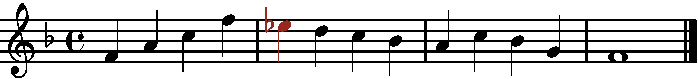
\includegraphics[width=0.8\linewidth]{t-exercice-reponse.cropped.pdf}\end{center}

\textbf{3.} 1~:~sol mixolydien, les notes de do majeur~; 2~:~la dorien, les notes de sol majeur~; 3~:~ré lydien, les notes de la majeur~; 4~:~do phrygien, les notes de la bémol majeur.

\end{remarque}

% =====================================================================
\section{Le fichier MusicXML}
\label{sec:musicxml}

Le fichier joint, \texttt{tonalites.musicxml}, fait entendre do majeur, son
relatif et son homonyme ; les deux modulations ; la mélodie transposée, avant
et après ; les sept modes sur les touches blanches, puis sur ré, du plus clair
au plus sombre ; enfin la mélodie de l'exercice de transposition. Le tout est
à la noire 80. Il se lit avec MuseScore, Finale, Sibelius, Dorico ou tout
éditeur de partitions ; sur slashbin.net, il s'écoute aussi dans Sodor Piano.

% =====================================================================
\section*{Colophon}
\addcontentsline{toc}{section}{Colophon}

Les gravures musicales sont produites par \textbf{LilyPond}, la composition
par \textbf{\LaTeX}. Les gravures, le cercle des quintes, le tableau des modes,
les réponses des exercices et le fichier MusicXML dérivent du modèle de
hauteurs des autres guides, les modules \texttt{gammes.py} et
\texttt{intervalles.py} du dossier \texttt{outils}. Avant d'écrire quoi que ce
soit, le générateur vérifie ce que le texte affirme : les trente tonalités et
leurs vingt-quatre sons, les notes modales seules à changer d'un mode à
l'autre, l'homonyme à trois altérations, les cinq tons voisins sur trois
armures et sur les degrés de la gamme, la sensible du ton d'arrivée dans
chaque modulation, la transposition qui conserve chaque intervalle et l'effet
de chaque altération, les tétracordes des modes et leur échelle sur ré. Pour
régénérer l'ensemble :

\begin{center}
\texttt{python3 outils/generer\_tonalites.py}\\
\texttt{(cd gravures \&\& lilypond -dcrop --formats=pdf t-*.ly)}\\
\texttt{pdflatex tonalites.tex}
\end{center}

\end{document}
